\documentclass[aspectratio=169,10pt]{beamer}

\usetheme{Madrid}
\usecolortheme{default}
\usefonttheme{professionalfonts}

\usepackage[utf8]{inputenc}
\usepackage[T1]{fontenc}
\usepackage[english]{babel}
\usepackage{amsmath,amssymb}
\usepackage{booktabs}
\usepackage{graphicx}
\usepackage{listings}
\usepackage{tikz}
\usepackage{pgfplots}
\pgfplotsset{compat=1.18}
\usepackage{xcolor}
\usepackage{array}
\usepackage{colortbl}

% Official Polytechnique colors
\definecolor{bleu303}{RGB}{0,62,92}
\definecolor{bleu303pale}{RGB}{204,221,230}
\definecolor{rouge485}{RGB}{213,43,30}
\definecolor{bleu315}{RGB}{0,104,128}

% Set Polytechnique style
\setbeamercolor{frametitle}{bg=bleu303, fg=white}
\setbeamercolor{title}{bg=bleu303, fg=white}
\setbeamercolor{subtitle}{fg=white}
\setbeamercolor{author}{fg=white}
\setbeamercolor{date}{fg=white}
\setbeamercolor{institute}{fg=white}
\setbeamercolor{block title}{bg=bleu303, fg=white}
\setbeamercolor{block body}{bg=bleu303pale, fg=black}
\setbeamercolor{alerted text}{fg=rouge485}
\setbeamercolor{example text}{fg=bleu315}
\setbeamercolor{section number projected}{bg=bleu303, fg=white}
\setbeamercolor{subsection number projected}{bg=bleu315, fg=white}
\setbeamercolor{item}{fg=bleu303}
\setbeamercolor{subitem}{fg=bleu315}
\setbeamercolor{subsubitem}{fg=rouge485}

\setbeamerfont{frametitle}{series=\bfseries}
\setbeamerfont{title}{series=\bfseries, size=\Large}
\setbeamerfont{subtitle}{series=\bfseries, size=\large}
\setbeamerfont{author}{series=\bfseries, size=\normalsize}
\setbeamerfont{date}{size=\normalsize}

% Custom title page template
\defbeamertemplate*{title page}{polytechnique}[1][]
{
  \begin{beamercolorbox}[sep=0pt, wd=\paperwidth, ht=\paperheight]{title}
    \begin{tikzpicture}[remember picture, overlay]
      \fill[bleu303] (current page.south west) rectangle (current page.north east);
    \end{tikzpicture}
    \centering
    \vspace*{2cm}
    {\usebeamerfont{title}\usebeamercolor[fg]{title}\inserttitle\par}
    \vspace*{0.5cm}
    {\usebeamerfont{subtitle}\usebeamercolor[fg]{subtitle}\insertsubtitle\par}
    \vspace*{2cm}
    {\usebeamerfont{author}\usebeamercolor[fg]{author}\insertauthor\par}
    \vspace*{0.5cm}
    {\usebeamerfont{date}\usebeamercolor[fg]{date}\insertdate\par}
  \end{beamercolorbox}
}

\lstset{
    basicstyle=\ttfamily\scriptsize,
    breaklines=true,
    backgroundcolor=\color{bleu303!5},
    keywordstyle=\color{bleu303}\bfseries,
    commentstyle=\color{bleu315}\itshape,
    frame=single,
    language=Python
}

\title[\textbf{RL for Block Blast}]{\textbf{Reinforcement Learning for Block Blast}}
\subtitle{From DQN to DVN to PPO + MCTS}
\author{Nathan Duboisset, Keyvan Attarian, Roman Lendormy, Arthur Fournier}
\date{March 2026}

\setbeamertemplate{title page}[polytechnique]

\AtBeginSection[]{
  \begin{frame}
    \frametitle{Outline}
    \tableofcontents[currentsection]
  \end{frame}
}

\begin{document}

%-----------------------------------------------------------------------------
\begin{frame}
\titlepage
\end{frame}

%-----------------------------------------------------------------------------
\begin{frame}{Outline}
\tableofcontents
\end{frame}

%=============================================================================
\section{The Game: Block Blast}

%-----------------------------------------------------------------------------
\begin{frame}{Block Blast: Overview}
\begin{columns}[T]
\begin{column}{0.55\textwidth}
\begin{block}{Game Rules}
\begin{itemize}
    \item $8\times8$ binary grid (0 = empty, 1 = filled)
    \item Place Tetromino-like pieces on the grid
    \item \textbf{Clearing}: any full row \emph{or} column is cleared
    \item \textbf{Game over}: no valid placements remain
\end{itemize}
\end{block}

\vspace{0.4em}
\begin{block}{7 Piece Shapes}
Dot, $2\times2$, $3\times3$, Line-3, Line-4, L-small, L-large\\
\footnotesize Each randomly rotated (0°, 90°, 180°, 270°)
\end{block}
\end{column}

\begin{column}{0.42\textwidth}
\begin{alertblock}{RL Challenges}
\begin{itemize}
    \item Long-horizon planning
    \item Large action space ($\leq 64$ / step)
    \item Sparse rewards
    \item Combinatorial structure (3P)
\end{itemize}
\end{alertblock}

\vspace{0.4em}
\begin{exampleblock}{Two Variants}
\begin{itemize}
    \item \textbf{1P}: one piece at a time
    \item \textbf{3P}: three pieces per round, free order
\end{itemize}
\end{exampleblock}
\end{column}
\end{columns}
\end{frame}

%-----------------------------------------------------------------------------
\begin{frame}{Block Blast: Example Board}
\begin{columns}[T]
\begin{column}{0.48\textwidth}
\begin{block}{1P Example}
\centering
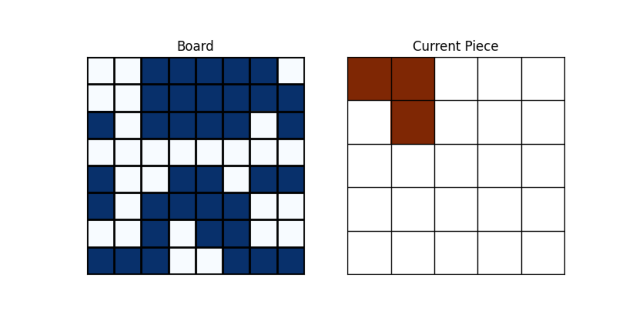
\includegraphics[width=0.95\linewidth]{board1p.png}
\end{block}
\end{column}

\begin{column}{0.48\textwidth}
\begin{block}{3P Example}
\centering
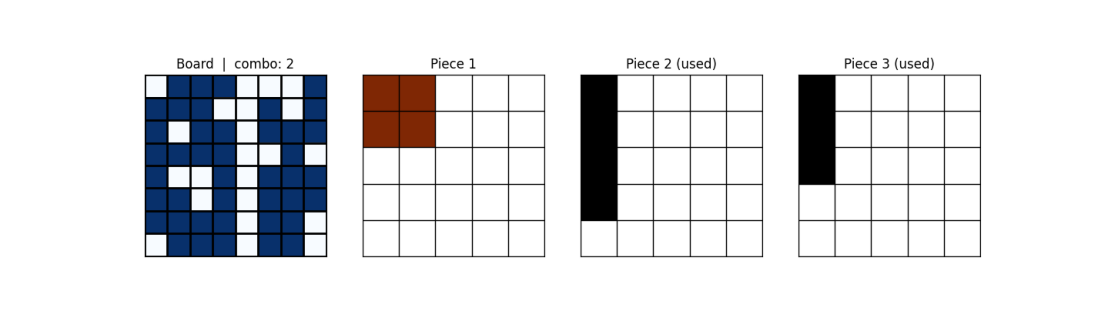
\includegraphics[width=0.95\linewidth]{board3p.png}
\end{block}
\end{column}
\end{columns}
\end{frame}

%-----------------------------------------------------------------------------
\begin{frame}{Environment: Single-Piece Variant (1P)}
\begin{columns}[T]
\begin{column}{0.48\textwidth}
\begin{block}{Observation (Dict)}
\begin{itemize}
    \item \texttt{board}: $8\times8$ int grid
    \item \texttt{piece}: $5\times5$ padded shape
    \item \texttt{valid\_placements}: $8\times8$ mask
    \item \texttt{placements\_result}: \emph{precomputed} $(8,8,8,8)$ afterstate tensor + reward map
\end{itemize}
\end{block}

\begin{block}{Action Space}
$\text{Discrete}(64)$ — action $a = 8r + c$\\
places piece top-left at $(r,c)$
\end{block}
\end{column}

\begin{column}{0.48\textwidth}
\begin{block}{Key Feature: Afterstates}
\vspace{0.3em}
The environment \textbf{precomputes} the resulting board for every valid placement before the agent acts.

\vspace{0.5em}
\[
\texttt{placements\_result}[r,c] = (s'_{r,c},\; r_{r,c})
\]
\vspace{0.3em}
This is the core enabler of the DVN approach.
\end{block}
\end{column}
\end{columns}
\end{frame}

%-----------------------------------------------------------------------------
\begin{frame}{Environment: Three-Piece Variant (3P)}
\begin{columns}[T]
\begin{column}{0.50\textwidth}
\begin{block}{3P Rules}
\begin{itemize}
    \item 3 pieces presented per \textbf{round}
    \item Agent plays all 3 in \textbf{any chosen order}
    \item \texttt{pieces\_used}: binary vector tracking played pieces
    \item \texttt{combo}: counter accumulating cleared lines across placements
\end{itemize}
\end{block}

\begin{block}{Action Space}
$\text{Discrete}(192) = \text{piece\_idx} \times 64 + r \times 8 + c$
\end{block}
\end{column}

\begin{column}{0.46\textwidth}
\begin{alertblock}{3P Lookahead API}
\texttt{get\_t\_plus\_3\_candidates($\gamma$)}
\vspace{0.3em}
\begin{itemize}
    \item Enumerates all $3! = 6$ orderings
    \item For each: all valid positions per piece
    \item Returns \emph{terminal board}, \emph{cumulative reward}, \emph{action sequence}
\end{itemize}
Used by the DVN 3P planner (see Section 4).
\end{alertblock}
\end{column}
\end{columns}
\end{frame}

%=============================================================================
\section{Reward Shaping}

%-----------------------------------------------------------------------------
\begin{frame}{Reward Shaping: First Attempt}
\begin{columns}[T]
\begin{column}{0.48\textwidth}
\begin{block}{Quadratic Combo Reward}
\[
r = b \cdot n_{\text{cleared}}^2, \quad b = 10
\]
\vspace{0.2em}
Intuition: strongly incentivise clearing multiple lines at once.
\end{block}

\vspace{0.5em}
\begin{exampleblock}{3P Variant (kept)}
\[
r = b \cdot (n_{\text{cleared}}^2 + \text{combo})
\]
The \texttt{combo} counter rewards sustained clearing streaks across rounds.
\end{exampleblock}
\end{column}

\begin{column}{0.48\textwidth}
\begin{alertblock}{Why It Failed for 1P}
\begin{itemize}
    \item Clearing $\geq 2$ lines at once is \textbf{rare early in training}
    \item Most steps give $r = 0$: \textbf{extremely sparse signal}
    \item Agent cannot learn what placement is ``good'' without feedback
    \item Training diverges or stalls
\end{itemize}
\end{alertblock}
\end{column}
\end{columns}
\end{frame}

%-----------------------------------------------------------------------------
\begin{frame}{Reward Shaping: Final Design (1P)}
\begin{block}{Final Reward Function}
\[
r = \underbrace{r_{\text{survive}}}_{5.0}
  + \underbrace{b \cdot n_{\text{cleared}}}_{10 \times \#\text{cleared lines}}
  + \underbrace{b \cdot \rho}_{\text{emptiness bonus}}
  - \underbrace{p_{\text{no3x3}}}_{20 \text{ if no free }3\times3}
\]
\end{block}

\begin{columns}[T]
\begin{column}{0.48\textwidth}
\begin{exampleblock}{Components}
\begin{itemize}
    \item $r_{\text{survive}} = 5$: reward for not dying
    \item $n_{\text{cleared}}$: rows + columns cleared
    \item $\rho \in [0,1]$: fraction of \textbf{empty cells} — keeps board clean
    \item $p_{\text{no3x3}} = 20$: penalty if no $3\times3$ empty window exists (``too full'')
\end{itemize}
\end{exampleblock}
\end{column}

\begin{column}{0.48\textwidth}
\begin{alertblock}{Invalid Move}
Penalty $-100$, \textbf{episode terminates}.
\end{alertblock}

\vspace{0.5em}
\begin{block}{Design Philosophy}
Dense signal at \emph{every} step, not just when lines clear. The emptiness ratio teaches the agent to \textbf{preserve space} for future pieces.
\end{block}
\end{column}
\end{columns}
\end{frame}

%=============================================================================
\section{DQN-Based Approaches}

%-----------------------------------------------------------------------------
\begin{frame}{DDQN and Rainbow: Architecture}
\begin{columns}[T]
\begin{column}{0.54\textwidth}
\begin{block}{\texttt{BlockBlastCNNNet1P} Backbone}
\begin{tabular}{ll}
\toprule
Layer & Output \\
\midrule
Board + mask $(2,8,8)$ & \\
Conv2d($2\to32$, $k=3$) & $32\times8\times8$ \\
Conv2d($32\to64$, $k=3$) & $64\times8\times8$ \\
Flatten & 4096 \\
\midrule
Piece $(1,5,5)$ & \\
Conv2d($1\to32$, $k=3$) & $32\times5\times5$ \\
Flatten & 800 \\
\midrule
Concat & 4896 \\
Linear $4896\to512\to256\to64$ & 64 Q-values \\
\bottomrule
\end{tabular}
\end{block}
\end{column}

\begin{column}{0.42\textwidth}
\begin{alertblock}{\textbf{2,674,464 parameters}}
\end{alertblock}

\vspace{0.5em}
\begin{block}{Rainbow Extensions}
\begin{enumerate}
    \item Distributional RL (C51, 51 atoms)
    \item Prioritized Replay (PER)
    \item N-step returns ($n=3$)
    \item Noisy Networks
    \item Dueling Architecture
\end{enumerate}
\end{block}
\end{column}
\end{columns}
\end{frame}

%-----------------------------------------------------------------------------
\begin{frame}{DQN: Why It Struggled}
\begin{alertblock}{Root Causes of Poor Performance}
\begin{enumerate}
    \item \textbf{Credit assignment}: a good placement may not clear a line for 3+ more steps. With $\gamma=0.99$, the discounted signal is weak over long horizons.

    \vspace{0.3em}
    \item \textbf{Q-function instability}: 64 action outputs, highly variable valid masks step-to-step. Q-values must track a non-stationary landscape.

    \vspace{0.3em}
    \item \textbf{Sample efficiency}: 2.67M parameters, only 1,000 training episodes. The model is severely underfit.

    \vspace{0.3em}
    \item \textbf{Perception overhead}: the network must simultaneously learn to recognise piece shapes, valid positions, \emph{and} long-term board value. This is a hard joint problem.
\end{enumerate}
\end{alertblock}

\begin{exampleblock}{Key Insight}
DQN treats this as a raw perception problem. We can do better by \textbf{leveraging the environment structure}.
\end{exampleblock}
\end{frame}

%-----------------------------------------------------------------------------
\begin{frame}{DQN Training Outcome (from report benchmark)}
\begin{columns}[T]
\begin{column}{0.58\textwidth}
\begin{center}
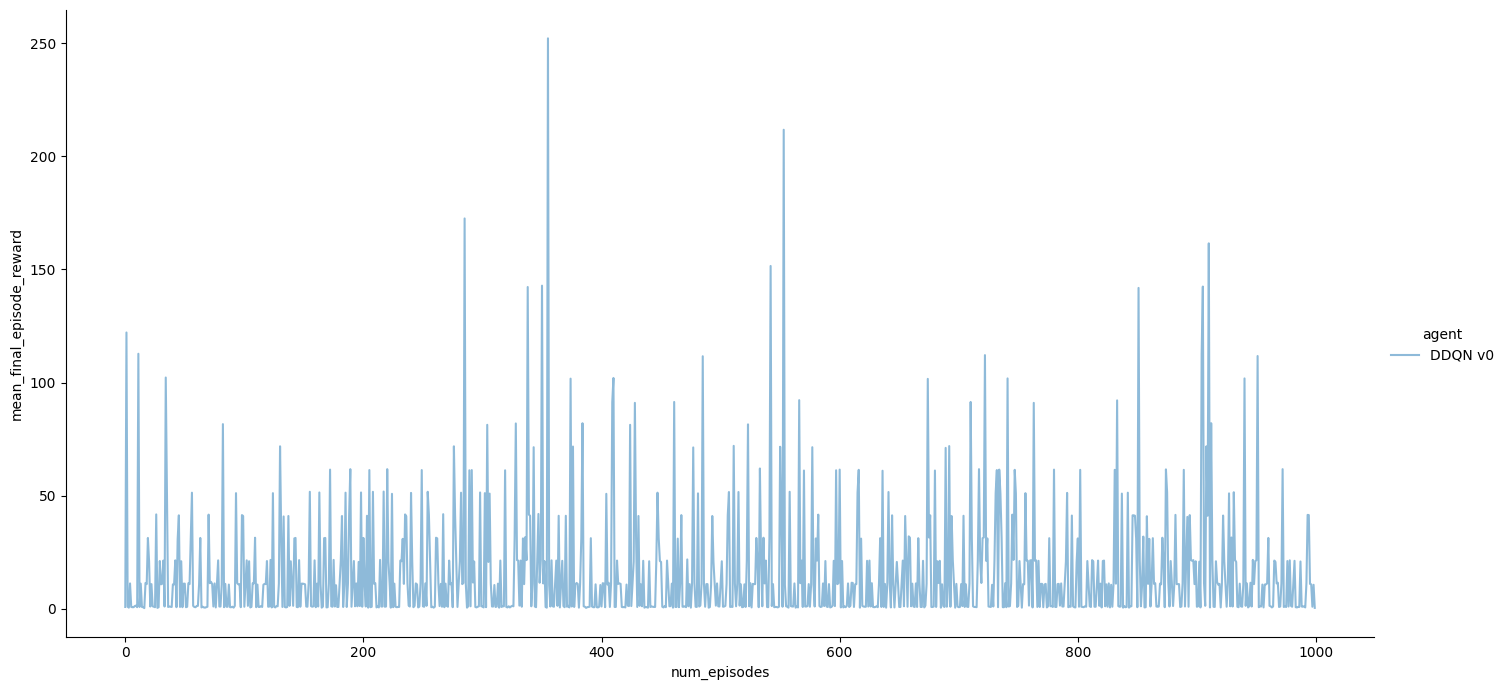
\includegraphics[width=0.98\textwidth]{traindqn.png}
\end{center}
\footnotesize DQN training figure (DDQN / Rainbow) from the report assets.
\end{column}

\begin{column}{0.38\textwidth}
\begin{alertblock}{Reading for DQN}
\begin{itemize}
    \item DDQN and Rainbow remained around \(\sim 20\) avg steps
    \item No stable long-game regime after 1,000 episodes
    \item Confirms underfitting and weak long-horizon credit assignment
\end{itemize}
\end{alertblock}
\end{column}
\end{columns}
\end{frame}

%=============================================================================
\section{Deep Value Network (DVN)}

%-----------------------------------------------------------------------------
\begin{frame}{DVN: Afterstate Formulation}
\begin{columns}[T]
\begin{column}{0.54\textwidth}
\begin{block}{Core Idea}
Instead of learning $Q(s, a)$, learn a \textbf{state value function}:
\[
V_\theta(s') \approx \text{long-term value of board } s'
\]
where $s'$ is the board \emph{after} placement and line clearing.
\end{block}

\vspace{0.5em}
\begin{block}{Action Selection (1-step lookahead)}
\[
a^* = \arg\max_a \left[ r_a + \gamma \cdot V_\theta(s'_a) \right]
\]
Enumerate all valid afterstates $\{s'_a, r_a\}$ via \texttt{placements\_result}, batch-evaluate $V_\theta$, pick best.
\end{block}
\end{column}

\begin{column}{0.42\textwidth}
\begin{exampleblock}{Advantages over DQN}
\begin{itemize}
    \item Network only evaluates \textbf{boards}, not (board, action) pairs
    \item Valid constraint handled implicitly
    \item Value captures board quality \textbf{independently of current piece}
    \item Much simpler function to learn
\end{itemize}
\end{exampleblock}

\begin{alertblock}{Key Requirement}
Environment must expose precomputed afterstates. Our \texttt{placements\_result} does exactly this.
\end{alertblock}
\end{column}
\end{columns}
\end{frame}

%-----------------------------------------------------------------------------
\begin{frame}{DVN Training Curves (W\&B)}
\begin{center}
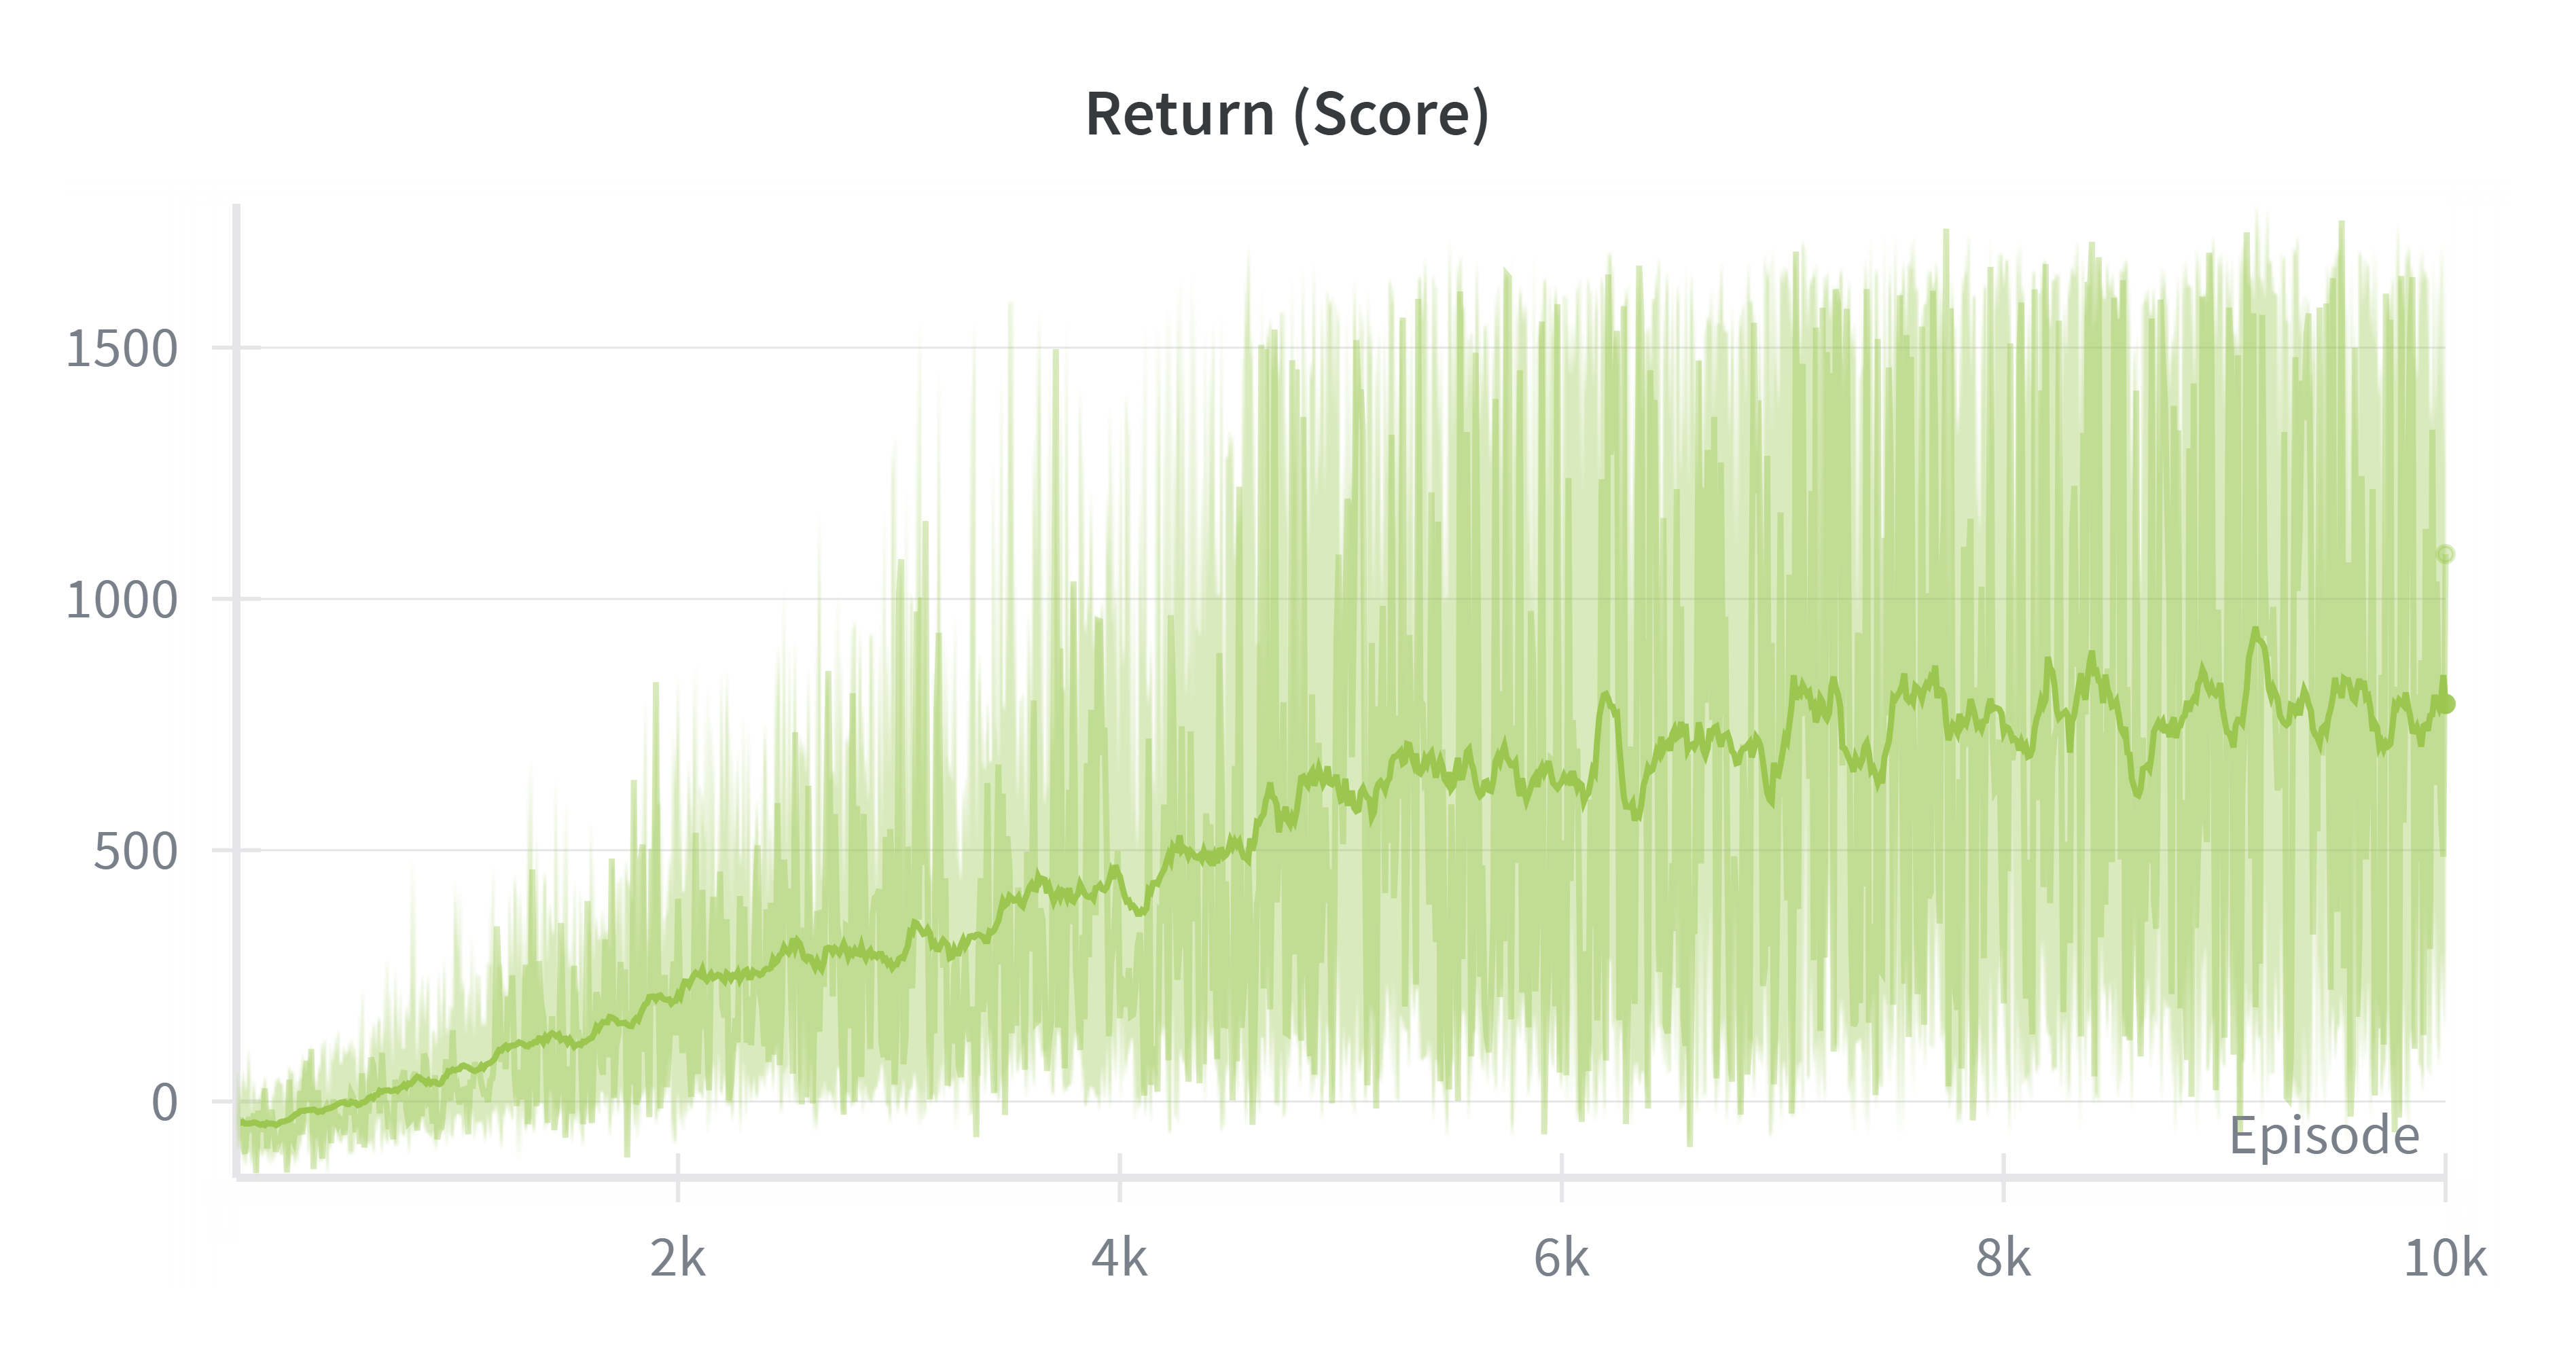
\includegraphics[width=0.31\textwidth]{../plots/wandb_reward.png}\hfill
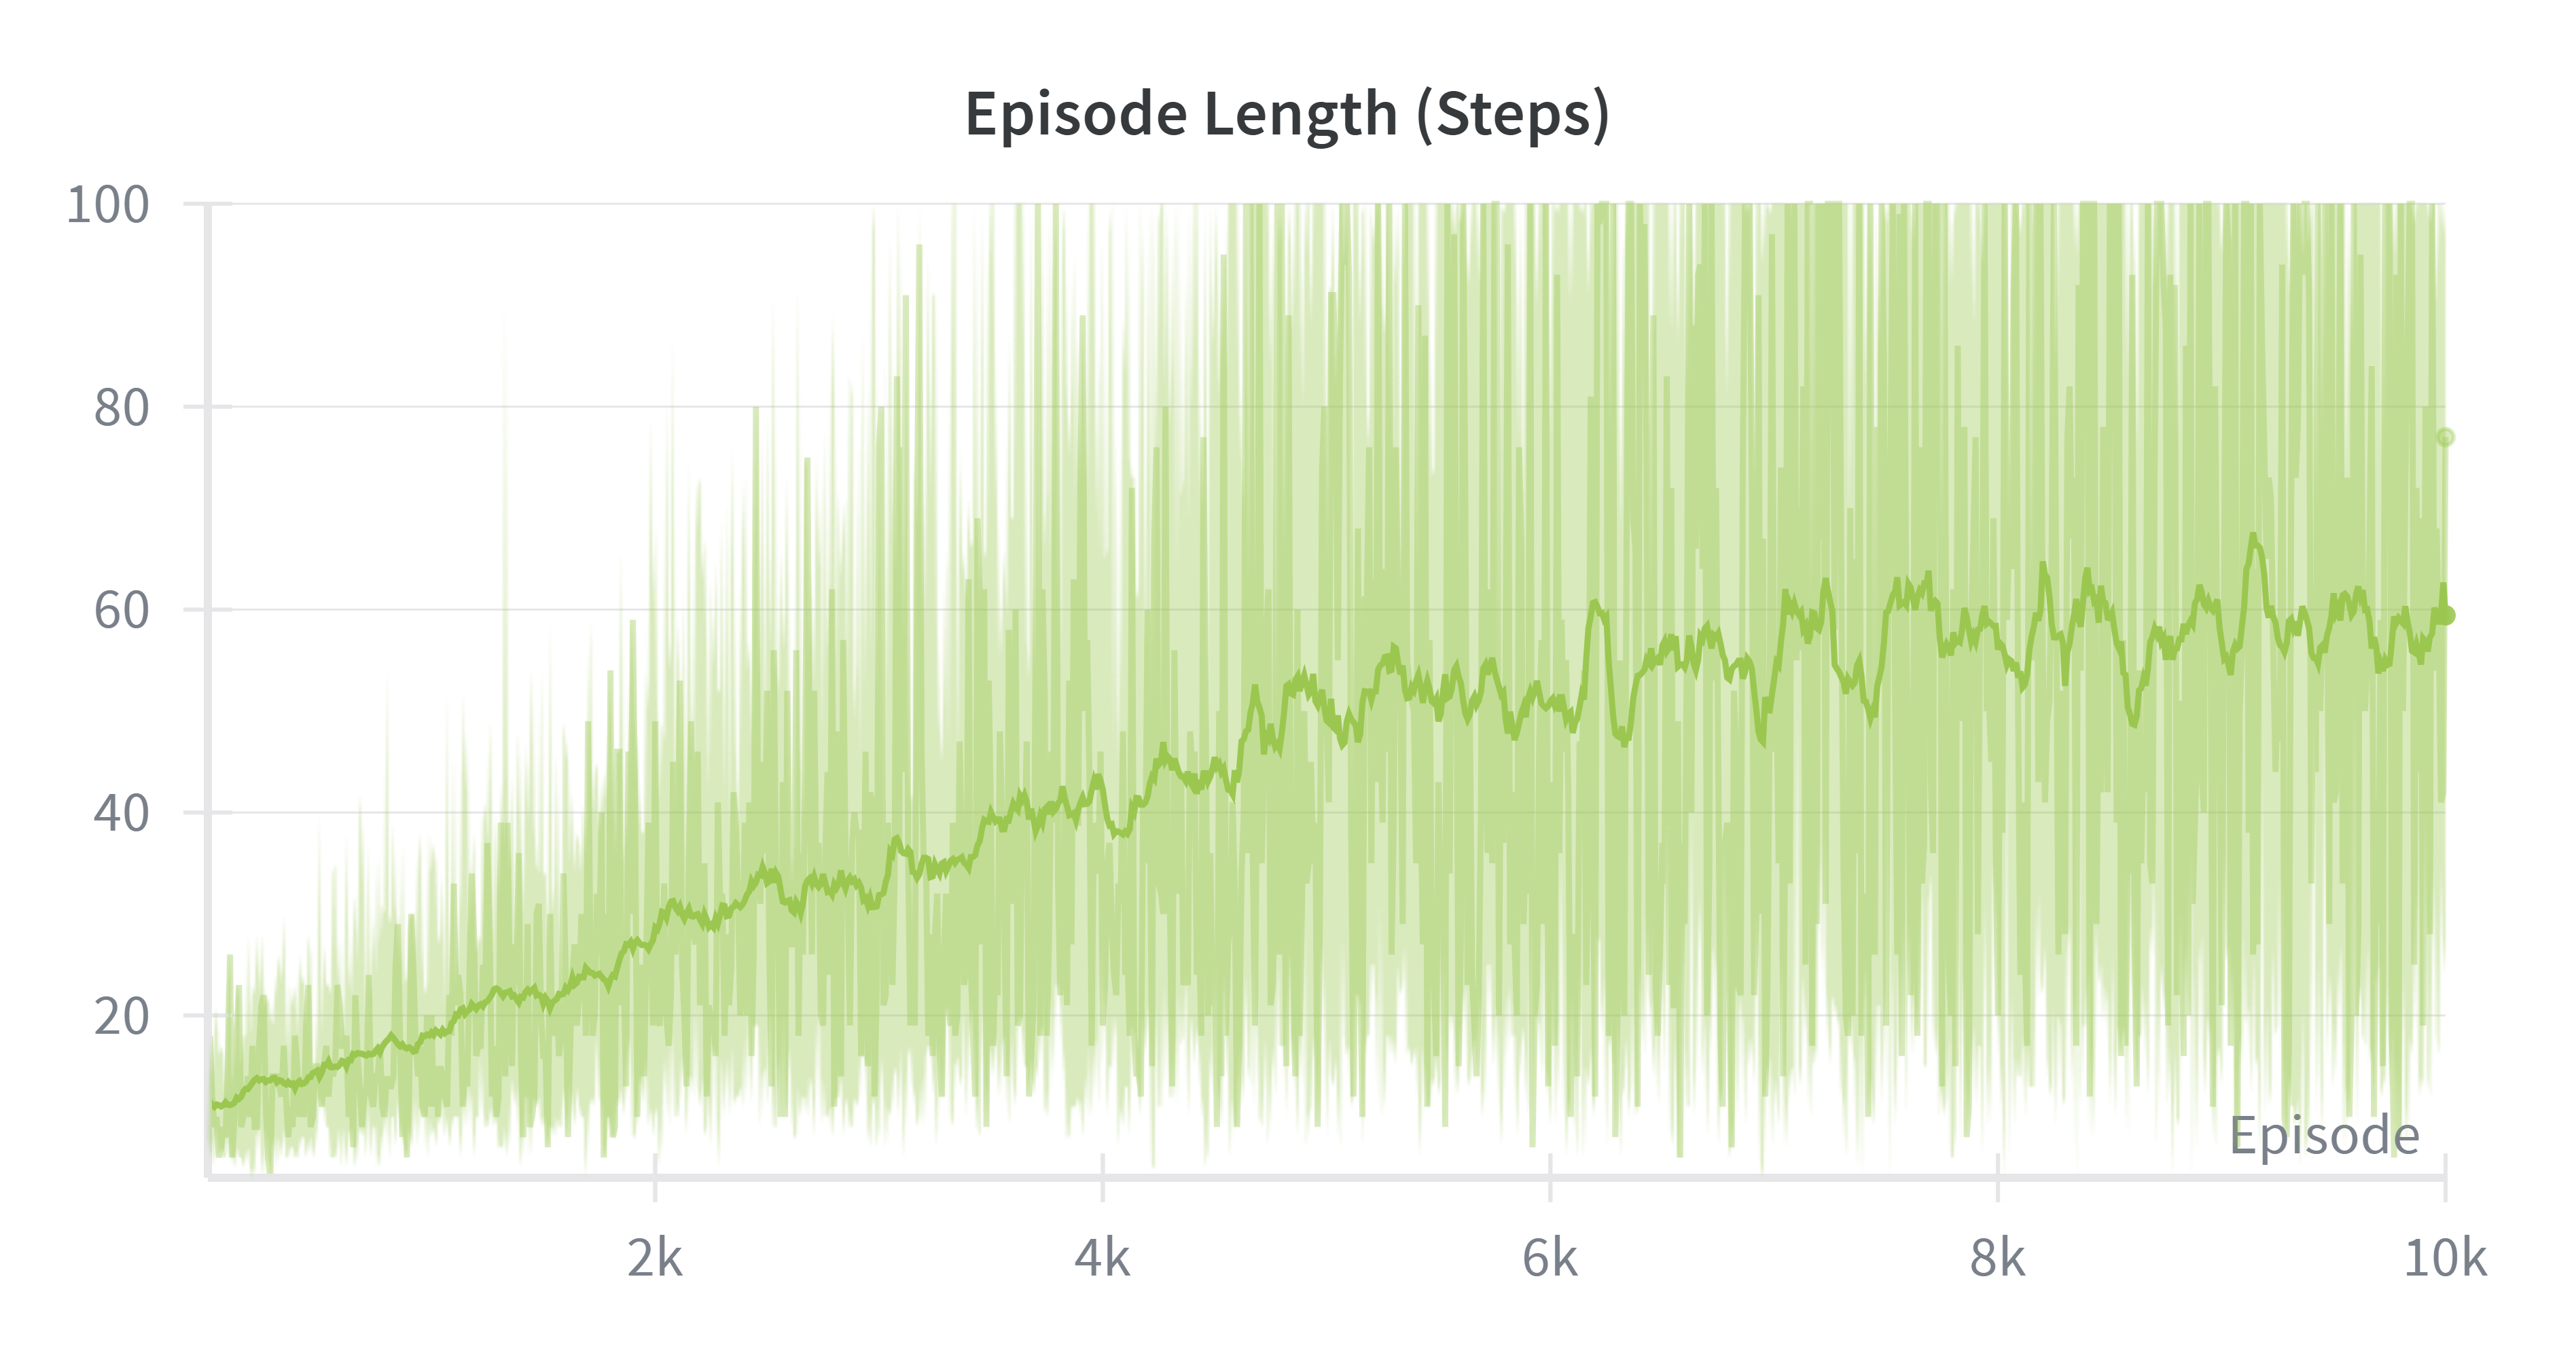
\includegraphics[width=0.31\textwidth]{../plots/wandb_loss.png}\hfill
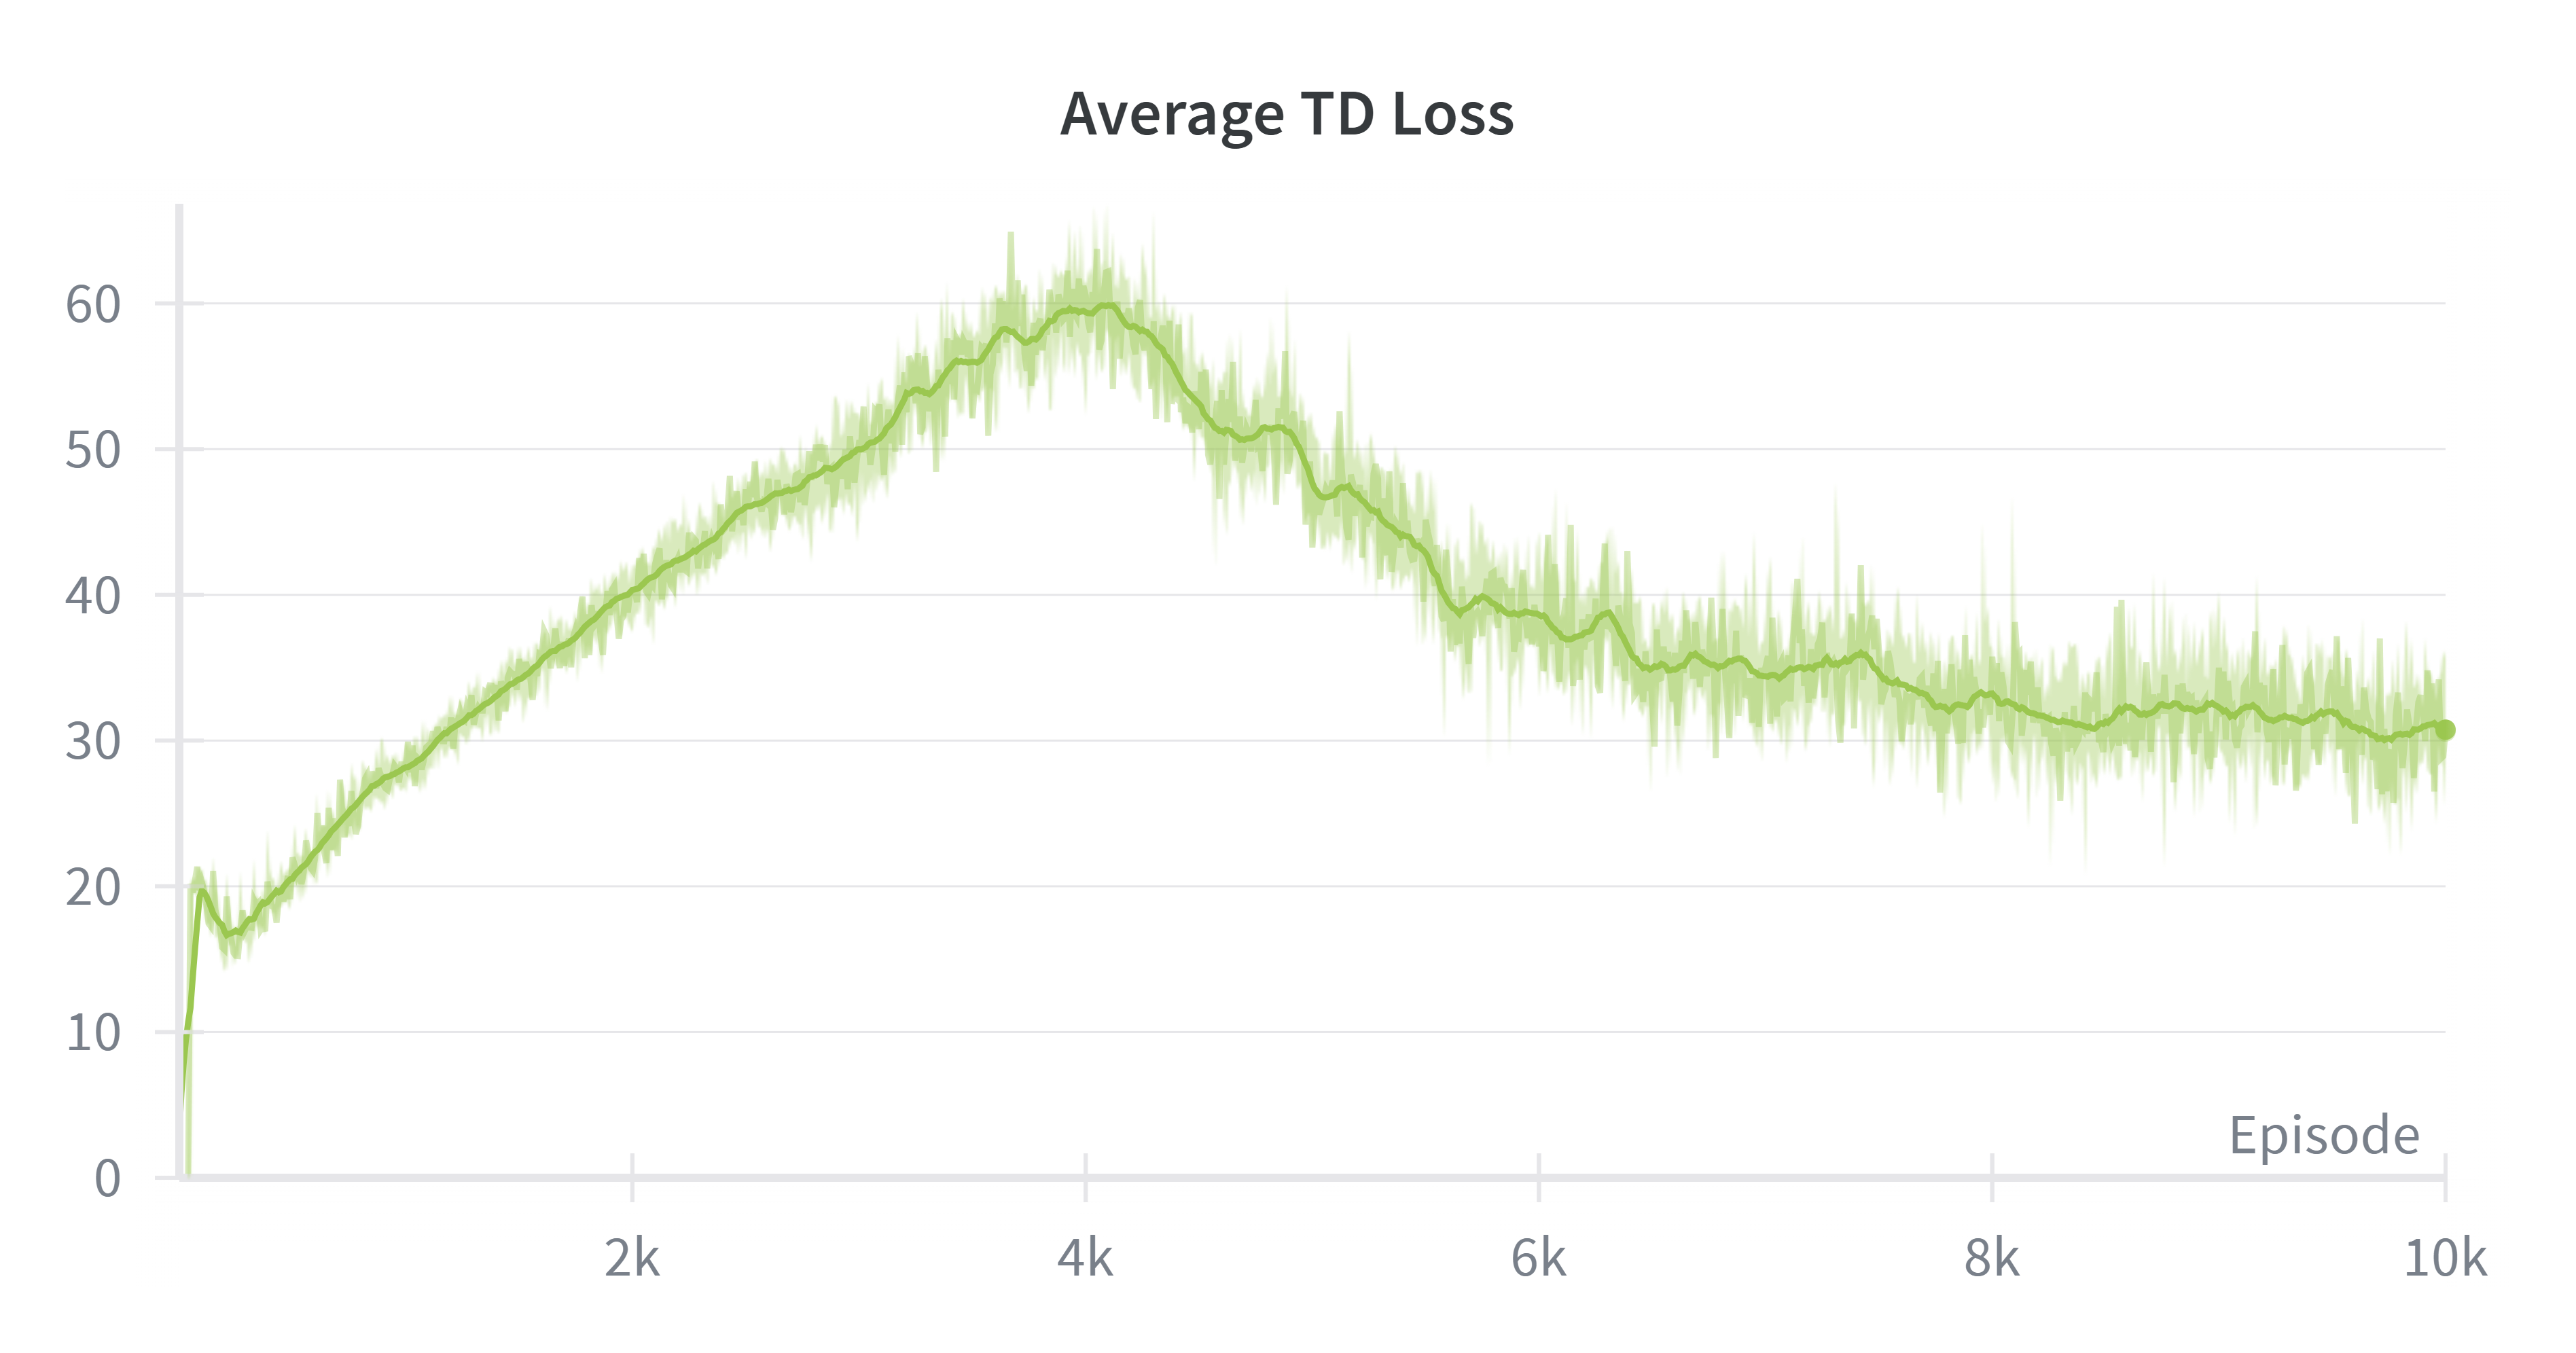
\includegraphics[width=0.31\textwidth]{../plots/wandb_eplen.png}
\end{center}

\vspace{0.4em}
\footnotesize
Left to right: reward, TD loss, and episode length versus training episodes (same figures as the report).
\end{frame}

%-----------------------------------------------------------------------------
\begin{frame}{DVN Architecture: Multi-Kernel CNN}
\begin{columns}[T]
\begin{column}{0.52\textwidth}
\begin{block}{8 Parallel Branches on $8\times8$ Board}
\footnotesize
\begin{tabular}{llcc}
\toprule
Kernel & Role & Filters & Pad \\
\midrule
$1\times1$  & Per-cell occupancy     & 1  & 0 \\
$2\times2$  & Small block patterns   & 8  & 1 \\
$3\times3$  & Piece-size patterns    & 16 & 1 \\
$4\times4$  & Medium structures      & 16 & 2 \\
$5\times5$  & Larger structures      & 16 & 2 \\
$8\times8$  & Global board summary   & 64 & 0 \\
$1\times8$  & \alert{Row detector}   & 4  & 0 \\
$8\times1$  & \alert{Column detector}& 4  & 0 \\
\bottomrule
\end{tabular}
\end{block}
\end{column}

\begin{column}{0.44\textwidth}
\begin{block}{Wall Padding}
Padding uses \texttt{ConstantPad2d} with value \textbf{1.0}: the kernel sees ``filled wall cells'' outside the grid boundary.

\vspace{0.3em}
\footnotesize No padding for line kernels ($1\times8$, $8\times1$).
\end{block}

\vspace{0.4em}
\begin{block}{Branch Output}
Each branch: Conv $\to$ LeakyReLU $\to$ Flatten $\to$ Linear$(\cdot\to16)$ $\to$ Linear$(16\to8)$

\vspace{0.3em}
Concat: $8 \times 8 = \mathbf{64}$ features
\end{block}
\end{column}
\end{columns}
\end{frame}

%-----------------------------------------------------------------------------
\begin{frame}{DVN Architecture: MLP Head \& Parameter Count}
\begin{columns}[T]
\begin{column}{0.50\textwidth}
\begin{block}{MLP Head}
\[
64 \xrightarrow{\text{Linear}} 64 \xrightarrow{\text{LReLU}} 16 \xrightarrow{\text{LReLU}} 1
\]
Scalar output: $V_\theta(s')$
\end{block}

\vspace{0.5em}
\begin{exampleblock}{Total: \textbf{42,461 parameters}}
$63\times$ fewer than DDQN/Rainbow!
\end{exampleblock}
\end{column}

\begin{column}{0.46\textwidth}
\begin{block}{Model Comparison}
\begin{tabular}{lc}
\toprule
Model & Params \\
\midrule
DDQN 1P   & 2,674,464 \\
Rainbow 1P & 2,674,464 \\
DDQN 3P   & 2,710,560 \\
\midrule
\textbf{DVN (ours)} & \textbf{42,461} \\
\bottomrule
\end{tabular}
\end{block}
\end{column}
\end{columns}

\vspace{0.5em}
\begin{exampleblock}{Why so small?}
The network only needs to answer: \emph{``Is this board position good for the long term?''} It does not need to reason about pieces, action encodings, or valid masks.
\end{exampleblock}
\end{frame}

%-----------------------------------------------------------------------------
\begin{frame}{DVN: Training}
\begin{columns}[T]
\begin{column}{0.50\textwidth}
\begin{block}{TD Learning on Afterstates}
\textbf{Target} (non-terminal):
\[
y_t = \max_{a'} \left[ r_{t+1,a'} + \gamma \cdot V_{\theta^-}(s'_{t+1,a'}) \right]
\]
\textbf{Target} (terminal):
\[
y_t = \frac{p_{\text{invalid}}}{\gamma}
\]
\textbf{Loss}: Huber (SmoothL1) + grad clip $\leq 10$
\end{block}
\end{column}

\begin{column}{0.46\textwidth}
\begin{block}{Training Protocol}
\begin{itemize}
    \item 10,000 episodes, max 100 steps
    \item $\varepsilon$: $1.0 \to 0.01$, decay $\times 0.999$/ep
    \item Buffer: 100,000 transitions
    \item Batch size: 128
    \item Adam, lr $= 10^{-4}$, StepLR
    \item Target net update: every 200 ep
    \item Logged via \textbf{Weights \& Biases}
    \item Checkpoints every 500 ep (full state)
\end{itemize}
\end{block}
\end{column}
\end{columns}
\end{frame}

%-----------------------------------------------------------------------------
\begin{frame}{DVN: 3P Planner}
\begin{columns}[T]
\begin{column}{0.54\textwidth}
\begin{block}{\texttt{RoundPlanner3P}}
At each new round:
\begin{enumerate}
    \item Call \texttt{get\_t\_plus\_3\_candidates($\gamma$)}
    \item Score each candidate sequence:
    \[
    \text{score} = R_{t+1:t+3} + \gamma^3 \cdot V_\theta(s_{t+3})
    \]
    \item Select \textbf{best 3-action sequence}
    \item Execute one action at a time
    \item \textbf{Replan} if an action becomes invalid
\end{enumerate}
\end{block}
\end{column}

\begin{column}{0.42\textwidth}
\begin{alertblock}{Computational Cost}
Full enumeration: $3! \times 64^3$ candidates in the worst case.
\vspace{0.3em}

Pure Python/NumPy: \textbf{very slow} for online evaluation.

\vspace{0.3em}
\textit{Future work}: batched GPU lookahead.
\end{alertblock}

\vspace{0.3em}
\begin{exampleblock}{Key Feature}
The DVN value function is \textbf{shared} between 1P and 3P — the planner is just a wrapper around the same $V_\theta$.
\end{exampleblock}
\end{column}
\end{columns}
\end{frame}

%=============================================================================
\section{Results}

%-----------------------------------------------------------------------------
\begin{frame}{Results: 1P Benchmark}
\begin{columns}[T]
\begin{column}{0.50\textwidth}
\begin{center}
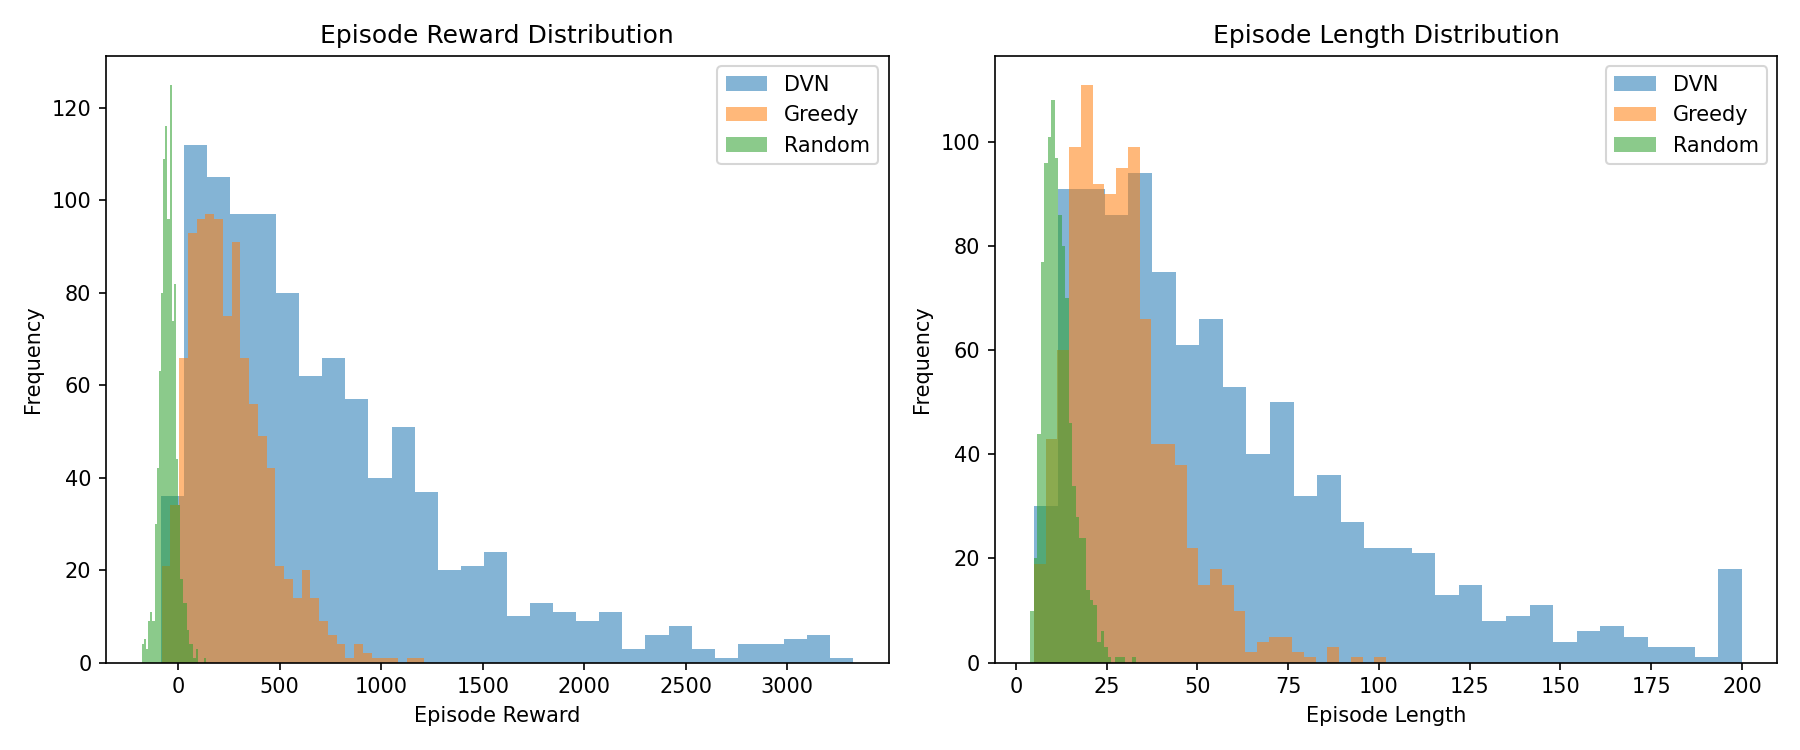
\includegraphics[width=0.95\textwidth]{../plots/benchmark_dvn_vs_greedy_vs_random_20260311_181312.png}
\end{center}
\footnotesize Episode steps (left) and return (right) over 200 episodes.
\end{column}

\begin{column}{0.46\textwidth}
\begin{tabular}{lcc}
\toprule
Agent & Avg Steps & Params \\
\midrule
Random      & $\sim$5  & --- \\
Greedy      & $\sim$30 & --- \\
DVN (untrained) & $\sim$20 & 42K \\
\textbf{DVN (trained)} & $\mathbf{\sim 60}$ & \textbf{42K} \\
DDQN 1P  & $\sim$20 & 2.67M \\
Rainbow  & $\sim$20 & 2.67M \\
\bottomrule
\end{tabular}

\vspace{0.5em}
\begin{exampleblock}{Key Result}
$63\times$ fewer parameters, better performance.
\end{exampleblock}
\end{column}
\end{columns}
\end{frame}

%-----------------------------------------------------------------------------
\begin{frame}{Results: 3P Benchmark (250 episodes, $\gamma=0.99$)}
\begin{columns}[T]
\begin{column}{0.54\textwidth}
\begin{block}{Performance Comparison}
\begin{tabular}{lcc}
\toprule
Agent & Mean Reward & Mean Steps \\
\midrule
Random & 25.33 & 11.93 \\
Greedy (D2) & 1\,884.90 & 44.45 \\
DVN (D2) & 23\,412.72 & 209.29 \\
DVN (D3) & 47\,469.39 & 223.72 \\
\bottomrule
\end{tabular}
\end{block}

\vspace{0.5em}
\begin{exampleblock}{Insights}
\begin{itemize}
    \item DVN depth-2: $\sim 5\times$ longer than greedy
    \item DVN depth-3: $\sim 480\times$ higher reward
    \item Preserved space wins over immediate lines
\end{itemize}
\end{exampleblock}
\end{column}

\begin{column}{0.42\textwidth}
\begin{alertblock}{Computational Cost}
Exhaustive enumeration: $3! \times 64^k$ candidates at depth $k$.

\vspace{0.3em}
Depth-3: very expensive without GPU batching.
\end{alertblock}
\end{column}
\end{columns}
\end{frame}

%=============================================================================
\section{Proximal Policy Optimization (PPO)}

%-----------------------------------------------------------------------------
\begin{frame}{PPO: A Stochastic Policy Approach}
\begin{columns}[T]
\begin{column}{0.54\textwidth}
\begin{block}{Architecture}
\begin{itemize}
    \item \textbf{BoardEncoder}: Conv stack on $8\times8$ $\to$ 128-d
    \item \textbf{PiecesEncoder}: 3 pieces $\to$ 64-d
    \item \textbf{ScalarEncoder}: combo, usage flags $\to$ 32-d
    \item \textbf{Trunk}: MLP $(224 \to 256)$
    \item \textbf{Heads}: policy $(256 \to 192)$ and value $(256 \to 1)$
\end{itemize}
\end{block}

\vspace{0.3em}
\begin{exampleblock}{Key Difference from DVN}
PPO conditions value on \textbf{full observation}: current board, all 3 pieces, piece usage, combo counter.
\end{exampleblock}
\end{column}

\begin{column}{0.42\textwidth}
\begin{block}{Training}
Clipped surrogate loss:
\[
L^{\text{CLIP}} = \mathbb{E}[\min(r_t \hat{A}_t, \text{clip}(r_t) \hat{A}_t)]
\]
where $r_t = \frac{\pi_\theta(a|s)}{\pi_{\theta_{\text{old}}}(a|s)}$

\vspace{0.3em}
Advantage $\hat{A}_t$ via GAE with value head.
\end{block}
\end{column}
\end{columns}
\end{frame}

%-----------------------------------------------------------------------------
\begin{frame}{PPO + MCTS Tree Search}
\begin{columns}[T]
\begin{column}{0.54\textwidth}
\begin{block}{Algorithm}
At each round (3 pieces):
\begin{enumerate}
    \item Enumerate all $3! \times 64^3$ candidate sequences
    \item Score each terminal state:
    \[
    \text{score} = \text{symlog}(\sum r_i) + \alpha \cdot \text{symlog}(V_\phi(s_{t+3}))
    \]
    \item Execute best 3-action sequence
    \item \textbf{Batch inference}: process 512 boards at a time on GPU
\end{enumerate}
\end{block}

\vspace{0.3em}
\begin{exampleblock}{Hyperparameter Sweep}
Optimal $\alpha \in [0.1, 0.5]$ balances immediate reward and value heuristic.
\end{exampleblock}
\end{column}

\begin{column}{0.42\textwidth}
\begin{alertblock}{Performance Gain}
\begin{itemize}
    \item \textbf{Baseline PPO}: $\sim$25 avg steps
    \item \textbf{PPO + MCTS}: $\sim$550 avg steps
    \item Cost: $\sim$1100 ms per round
\end{itemize}
\end{alertblock}

\end{column}
\end{columns}
\end{frame}

%-----------------------------------------------------------------------------
\begin{frame}{PPO Training Curves (Loss)}
\begin{center}
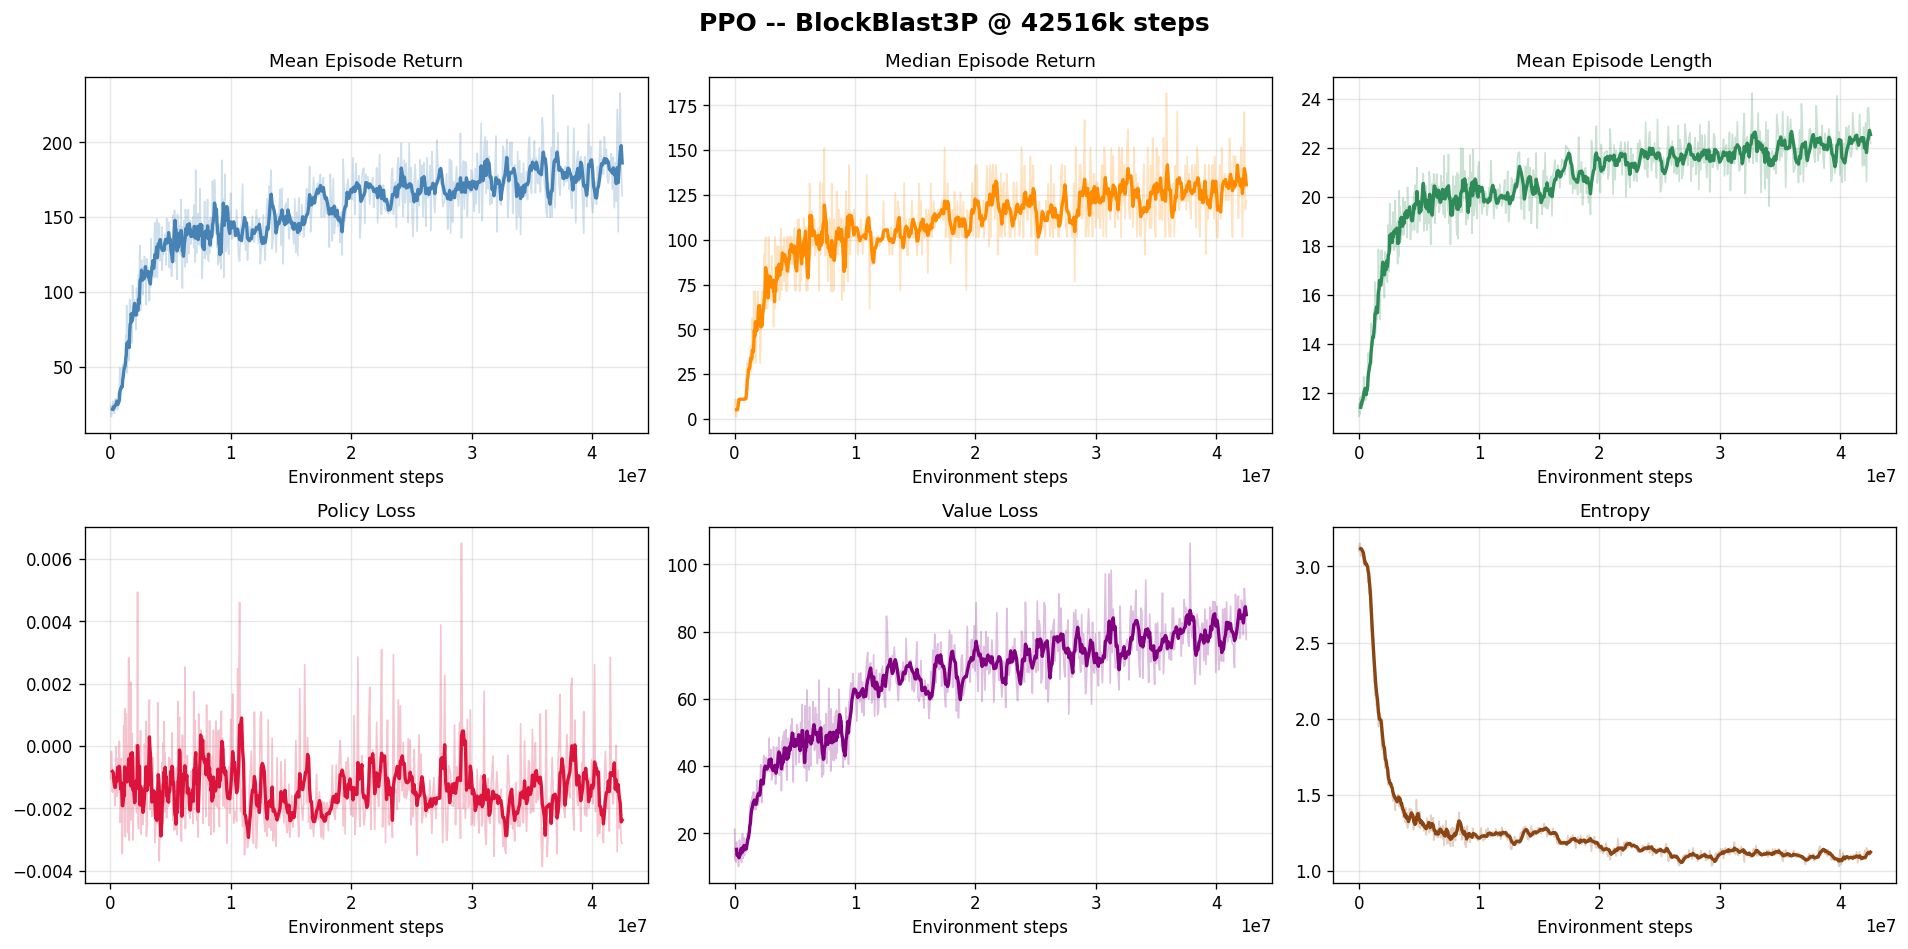
\includegraphics[width=0.90\textwidth]{../plots/ckpt_42516k_curves.png}
\end{center}

\vspace{0.3em}
\footnotesize
Loss curves from PPO training checkpoints (\texttt{ckpt\_...}).
\end{frame}

%=============================================================================
\section{Discussion \& Future Work}

%-----------------------------------------------------------------------------
\begin{frame}{DVN vs.\ DQN vs.\ PPO}
\begin{columns}[T]
\begin{column}{0.54\textwidth}
\begin{exampleblock}{Why DVN $>$ DQN}
\begin{itemize}
    \item Decouples \emph{``board state''} from \emph{``action selection''}
    \item No need to reason about piece geometry
    \item Simpler learning objective $\Rightarrow$ sample-efficient
    \item Valid constraints implicit
\end{itemize}
\end{exampleblock}

\vspace{0.3em}
\begin{exampleblock}{Why PPO $>$ DVN (with MCTS)}
\begin{itemize}
    \item Full observation conditioning: sees all pieces + state
    \item Richer value heuristic for search
    \item Stochastic policy naturally explores
    \item MCTS exhaustive evaluation within depth
\end{itemize}
\end{exampleblock}
\end{column}

\begin{column}{0.42\textwidth}
\begin{alertblock}{Limitations}
\begin{itemize}
    \item DVN: piece-agnostic, limited lookahead
    \item PPO+MCTS: $O(3! \times 64^k)$ enumeration cost
    \item Piece randomness: truly random (harder than real game)
\end{itemize}
\end{alertblock}
\end{column}
\end{columns}
\end{frame}

%-----------------------------------------------------------------------------
\begin{frame}{Future Work}
\begin{block}{Short-term Improvements}
\begin{itemize}
    \item Encode \textbf{next pieces} as input channels for DVN
    \item Hand-crafted features: hole count, row/column density, height variance (Tetris-inspired)
    \item \textbf{GPU-batched lookahead} for faster 3P evaluation
\end{itemize}
\end{block}

\vspace{0.5em}
\begin{block}{Longer-term Research}
\begin{itemize}
    \item \textbf{Curriculum learning}: progressively harder piece distributions
    \item \textbf{Model-based RL}: learn transition model for deeper planning
    \item \textbf{Hybrid}: combine PPO stochasticity with DVN piece-agnostic structure
\end{itemize}
\end{block}
\end{frame}

%-----------------------------------------------------------------------------
\begin{frame}{Conclusion}
\begin{block}{Key Takeaways}
\begin{enumerate}
    \item \textbf{Environment design}: precomputed afterstates unlock efficient RL approaches
    
    \vspace{0.3em}
    \item \textbf{Reward shaping matters}: sparse quadratic bonus $\to$ dense survival + emptiness bonus
    
    \vspace{0.3em}
    \item \textbf{DVN}: 42K parameters, $63\times$ smaller than DQN/Rainbow, achieves $\sim$60 steps via structure exploitation
    
    \vspace{0.3em}
    \item \textbf{PPO + MCTS}: $\sim$550 steps via tree search + learned value heuristic (limited by enumeration cost)
    
    \vspace{0.3em}
    \item \textbf{Lesson}: Leverage environment structure $>$ bigger models
\end{enumerate}
\end{block}

\vspace{0.8em}
\centering
\normalsize
\textbf{From Deep Q-Networks to Value Functions to Guided Tree Search}
\end{frame}

%-----------------------------------------------------------------------------
\appendix
\begin{frame}{Appendix: Benchmark (Earlier Run)}
\begin{center}
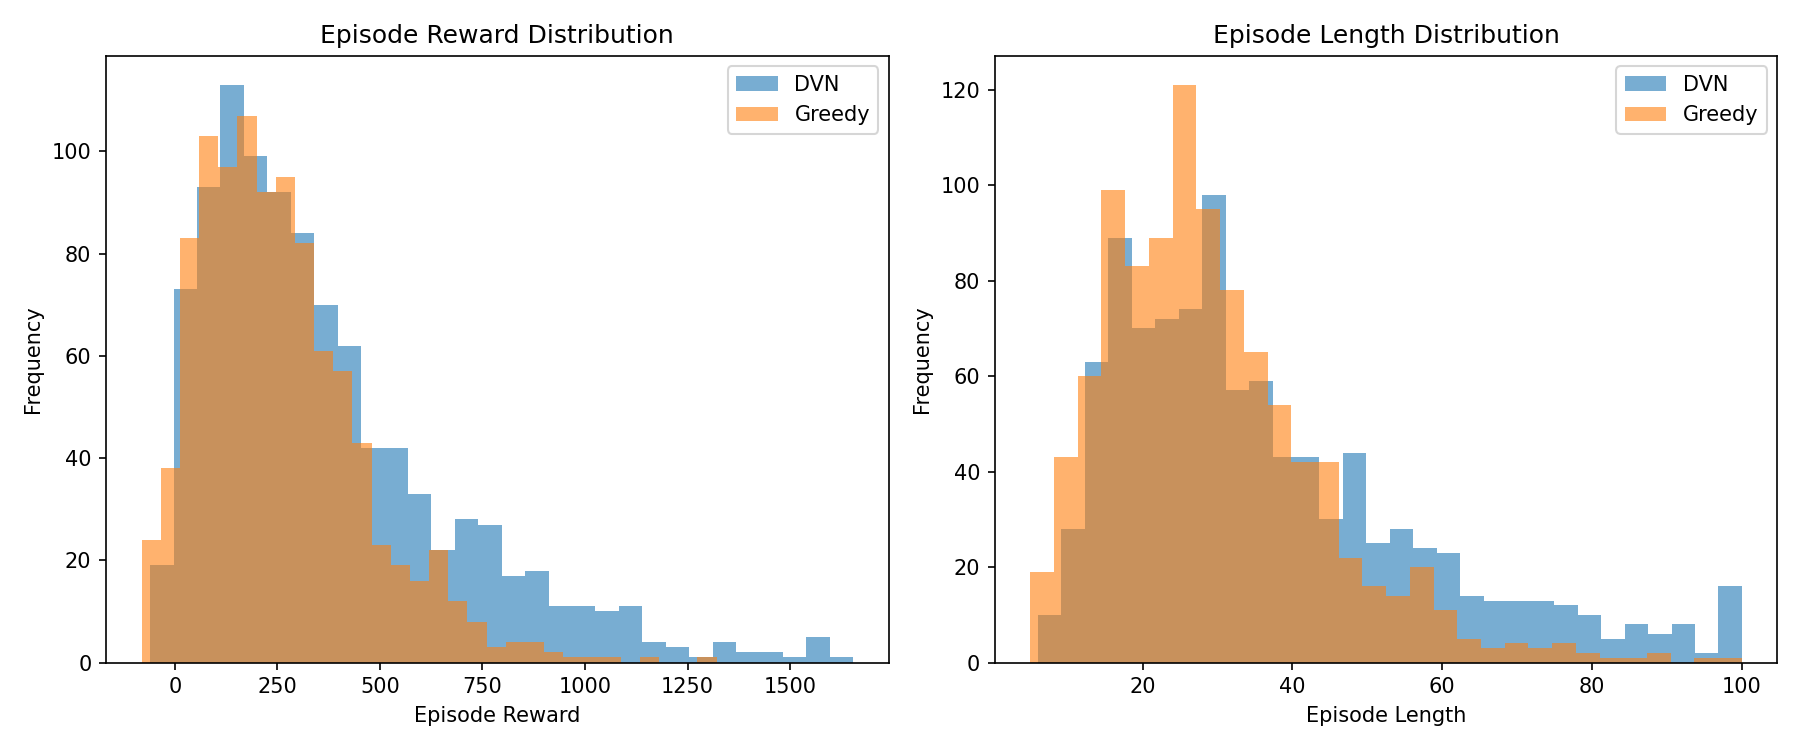
\includegraphics[width=0.72\textwidth]{../plots/benchmark_dvn_vs_greedy_20260311_123451.png}
\end{center}
\footnotesize Earlier benchmark comparing DVN vs.\ greedy only (before random baseline was added).
\end{frame}

\begin{frame}{Appendix: DVN Training Algorithm}
\begin{columns}[T]
\begin{column}{0.54\textwidth}
\begin{block}{Algorithm (simplified)}
\footnotesize
\textbf{Input:} $V_\theta$, target $V_{\theta^-}$, env, buffer $\mathcal{B}$\\[0.3em]
\textbf{For} each episode:\\
\quad \textbf{For} each step $t$:\\
\quad\quad Compute all afterstates $\{(s'_a, r_a)\}$\\
\quad\quad $a^* = \arg\max_a [r_a + \gamma V_\theta(s'_a)]$ (greedy)\\
\quad\quad or sample random (exploration)\\
\quad\quad Store $(s'_{a^*}, r_{a^*}, s_{\text{next}}, \text{done})$ in $\mathcal{B}$\\
\quad\quad Sample batch from $\mathcal{B}$\\
\quad\quad Compute TD targets $y_t$\\
\quad\quad Update $\theta$ via Huber loss\\
\quad Periodically: $\theta^- \leftarrow \theta$
\end{block}
\end{column}

\begin{column}{0.42\textwidth}
\begin{block}{Hyperparameters}
\begin{tabular}{ll}
\toprule
Param & Value \\
\midrule
$\gamma$ & 0.99 \\
$\varepsilon_0 \to \varepsilon_{\min}$ & $1.0 \to 0.01$ \\
Buffer size & 100,000 \\
Batch size & 128 \\
LR & $10^{-4}$ \\
Target update & 200 ep \\
\bottomrule
\end{tabular}
\end{block}
\end{column}
\end{columns}
\end{frame}

\end{document}
